%% ====================================================================
%% The HPC: what it is, connecting, working on it
%% ====================================================================

\section[HPC]{What is the HPC?}

\begin{frame}{What is the HPC?}
\small
\begin{itemize}
    \item HPC stands for high-performance computing
    \item The HPC is a cluster of computers that work together as a single system
    \item The computers run Rocky Linux
    \item It is shared by many groups, and managed through Slurm
\end{itemize}
\medskip
\begin{columns}[b,onlytextwidth]
    \column{0.3\textwidth}
    \centering
    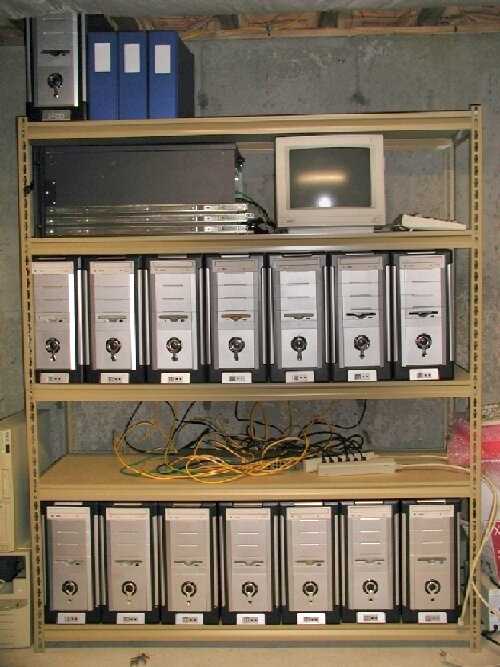
\includegraphics[height=2.9cm]{beowulf.jpg}\par
    \footnotesize The idea: ordinary PCs, connected
    \column{0.66\textwidth}
    \centering
    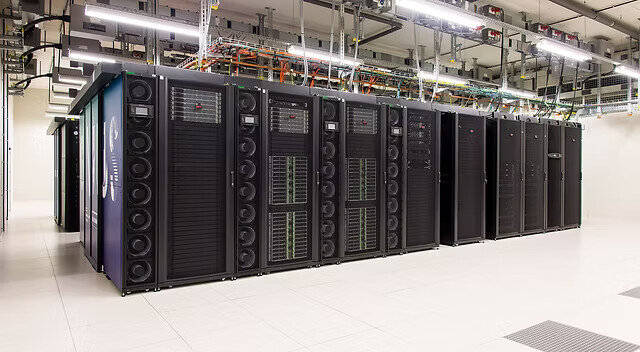
\includegraphics[height=2.9cm]{hpc_pro.jpg}\par
    \footnotesize Today: racks of servers in a data centre
\end{columns}
\end{frame}

\begin{frame}{Who makes use of the HPC?}
\begin{itemize}
    \item University Medical Center Utrecht
          \begin{itemize}
              \item Division Biomedical
              \item Division Cardiology \& Pulmonology
              \item Division Imaging
              \item Division Internal Medicine
              \item Julius Center
              \item Division Laboratories \& Pharmacy
              \item Division Neuroscience
          \end{itemize}
    \item Utrecht University
          \begin{itemize}
              \item Science Faculty, Department of Information and Computing Sciences
              \item Science Faculty, Department of Biology
          \end{itemize}
    \item Hubrecht Institute
    \item Princess Máxima Center for Pediatric Oncology
\end{itemize}
\end{frame}

\begin{frame}{An HPC node is a much bigger computer than your laptop}
\small
\begin{cmdtable}{llll}
               & \textbf{My UMC laptop} & \textbf{One HPC node} & \textbf{The cluster} \\
    \midrule
    CPU cores  & 8 (Apple M3)           & 24--48                & 2172 in 57 nodes     \\
    Memory     & 8 GB                   & 256 GB -- 1 TB        &                      \\
    Local disk & 560 GB SSD             & 1--2 TB tmpspace      & + shared storage     \\
\end{cmdtable}

\bigskip
\begin{itemize}
    \item \textbf{Core}: does one computation at a time. 8 cores: 8 things at once
    \item \textbf{Memory} (RAM): where data sits while it is being worked on.
          Fast, but temporary
    \item \textbf{Disk}: where your files are kept, even when the computer is off
\end{itemize}
\end{frame}

\begin{frame}{Login, compute and transfer nodes}
\begin{columns}[c]
    \column{0.42\textwidth}
    \small
    \begin{itemize}
        \item \textbf{Login nodes} (\cmd{hpcs05}, \cmd{hpcs06}): log in, edit scripts, submit jobs.
              \alert{Never run analyses here}
        \item \textbf{Compute nodes} (57): where your jobs run.
              You get there through Slurm
        \item \textbf{Transfer nodes} (\cmd{hpct04}, \cmd{hpct05}): move data to and from the HPC
        \item \textbf{Shared storage}: every node sees the same files
    \end{itemize}
    \column{0.56\textwidth}
    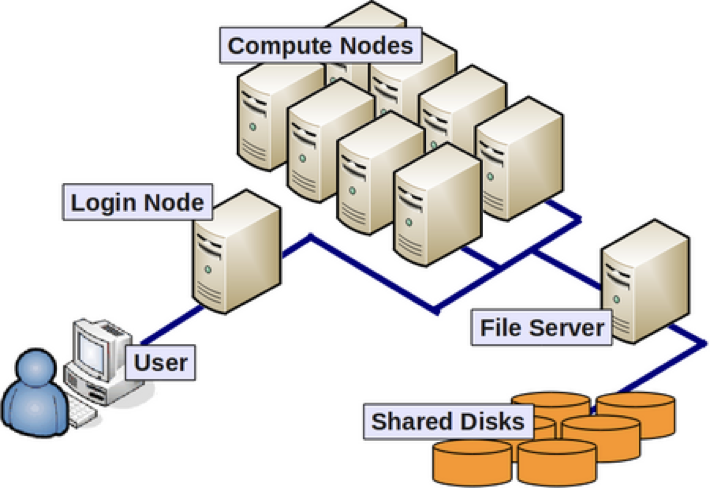
\includegraphics[width=\linewidth]{cluster_draw.png}
\end{columns}
\end{frame}

\begin{frame}{Slurm decides who runs what, and where}
\begin{itemize}
    \item The HPC is shared: hundreds of users, one set of nodes
    \item You ask Slurm for resources: cores, memory, time, disk space
    \item Your job waits in a queue until a node with those resources is free
    \item Fair share: if your group used little recently, your jobs start sooner
    \item Small, short requests find a free spot faster
\end{itemize}
\end{frame}

\begin{frame}{Where to keep your files on the HPC}
\small
\begin{cmdtablex}{lllL}
    \textbf{Where} & \textbf{Path}              & \textbf{Size} & \textbf{Use it for}                         \\
    \midrule
    Home           & \cmd{/home/<group>/<user>} & 7 GB          & Scripts, settings                           \\
    Project        & \cmd{/hpc/<group>/<user>}  & Group's       & Data, results, Conda envs                   \\
    tmpspace       & \cmd{/scratch/<jobid>}     & Requested     & Fast disk during a job, on the compute node \\
\end{cmdtablex}

\medskip
\small
\begin{itemize}
    \item Your home directory is small: keep big data in the project directory
    \item Project quota (several TB) is shared by your group: use at most 1 TB yourself
    \item tmpspace is deleted when the job ends: copy your results back
    \item \alert{There are no backups}: keep a copy of your raw data elsewhere, and your scripts in Git
\end{itemize}
\end{frame}

\section[Connecting]{Connecting to the HPC}
\begin{frame}{Using Open OnDemand}
\small
\hint{From here on: type along if you have HPC access, otherwise follow on the screen}
\par\medskip
Open OnDemand is a web portal to the HPC: browse files, open a terminal, or start RStudio and Jupyter, all in your browser.
Go to one of:

\begin{itemize}
    \item \cmd{https://hpcs05.op.umcutrecht.nl}
    \item \cmd{https://hpcs06.op.umcutrecht.nl}
\end{itemize}

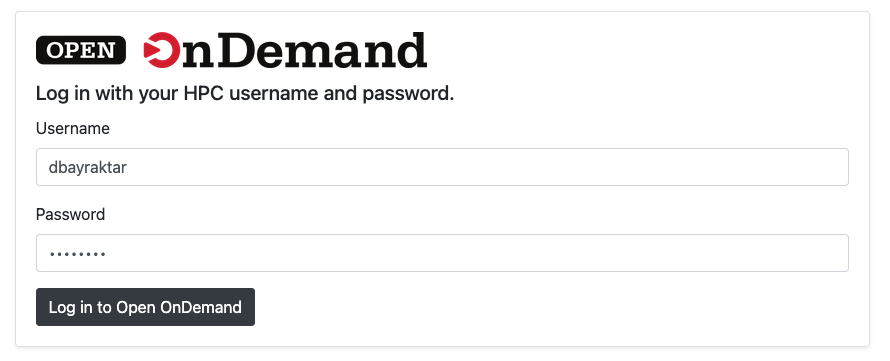
\includegraphics[width=\linewidth]{ondemand1.png}
\end{frame}

\begin{frame}[fragile]{Optional: log in from your own terminal}
\small
Not needed today: Open OnDemand is enough. Later, for \cmd{ssh} and \cmd{rsync} from your laptop:
\begin{enumerate}
    \item Make a separate key for the HPC, with a passphrase
    \item Log in with that key; the first time, type \cmd{yes}
\end{enumerate}
\begin{lstlisting}
ssh-keygen -t ed25519 -C "HPC" -f ~/.ssh/id_ed25519_hpc
ssh -i ~/.ssh/id_ed25519_hpc \
    <user>@hpcs05.op.umcutrecht.nl
\end{lstlisting}
\hint{Already have \cmd{~/.ssh/id_ed25519_hpc}? Keep using it}
\end{frame}

\begin{frame}[fragile]{Moving data to and from the HPC}
\small
\begin{itemize}
    \item Use the \textbf{transfer nodes} for data: not the login nodes
    \item \cmd{rsync} only copies what changed, and can continue after a broken connection
    \item Check big transfers with \cmd{md5sum} afterwards
\end{itemize}
\begin{lstlisting}[style=footnotesize]
# from your laptop to the HPC
rsync -av --progress -e "ssh -i ~/.ssh/id_ed25519_hpc" data/ \
    <user>@hpct04.op.umcutrecht.nl:/hpc/<group>/<user>/data/

# from the HPC back to your laptop
rsync -av -e "ssh -i ~/.ssh/id_ed25519_hpc" \
    <user>@hpct04.op.umcutrecht.nl:/hpc/<group>/<user>/results/ \
    results/
\end{lstlisting}
\hint{The trailing \cmd{/} matters: \cmd{data/} copies what is \emph{in} \cmd{data}.
    Needs the HPC key from the optional slide; without it, use the file browser in Open OnDemand}
\end{frame}

\begin{frame}{Exercises: moving data}
\begin{exlist}{4_hpc.md}
    \ex{4.1}{Copy with rsync}{1}
    \ex{4.2}{Copy again}{1}
    \ex{4.3}{Check the copy}{2}
\end{exlist}
\end{frame}

\section[Working]{Working on the HPC}
\begin{frame}{Asking Slurm for resources}
\small
\begin{cmdtable}{lll}
    \textbf{Option}                 & \textbf{You ask for}      & \textbf{Example}          \\
    \midrule
    \cmd{-c}, \cmd{--cpus-per-task} & CPU cores                 & \cmd{-c 4}                \\
    \cmd{--mem}                     & Memory                    & \cmd{--mem=8G}            \\
    \cmd{--time}                    & Time limit               & \cmd{--time=02:00:00}     \\
    \cmd{--gres=tmpspace:<size>}    & Local disk               & \cmd{--gres=tmpspace:50G} \\
    \cmd{-A}, \cmd{--account}       & Group account            & \cmd{-A <account>}        \\
\end{cmdtable}

\bigskip
\begin{itemize}
    \item These are limits: use more memory or time, and Slurm stops your job
    \item The job then ends as \cmd{OUT_OF_MEMORY} or \cmd{TIMEOUT}
\end{itemize}
\end{frame}

\begin{frame}[fragile]{Using \cmd{srun} for interactive sessions}
Requesting an interactive job:
\begin{lstlisting}
srun -c 2 --mem=4G --time=01:00:00 --pty bash
\end{lstlisting}
\begin{itemize}
    \item \cmd{--pty bash}: give me a terminal on the compute node
    \item Slurm finds a node, and your prompt changes to that node's name
    \item Everything you run now uses the requested resources
    \item Type \cmd{exit} when you are done: the resources go back to the pool
\end{itemize}
\end{frame}

\begin{frame}[fragile]{Demo: from the login node to a compute node}
\begin{lstlisting}[style=footnotesize]
# in a terminal in Open OnDemand
hostname                    # hpcs05: the login node
cd /hpc/<group>/<user>/data/HPC_intro/exercise_data

srun -c 1 --mem=1G --time=00:30:00 --pty bash
hostname                    # n0...: a compute node
grep -c "^>" */assembly.fasta
exit                        # back on the login node
\end{lstlisting}
\end{frame}

\begin{frame}[fragile]{Conda on the HPC}
\small
\begin{itemize}
    \item Environments are large: keep them out of your home directory, or you will hit its quota
    \item Install Miniforge itself in \cmd{/hpc/<group>/<user>/data/miniforge3} too: the installer asks where
    \item Install and run tools on a compute node, not on the login node (\cmd{srun})
\end{itemize}
\begin{lstlisting}[style=footnotesize]
conda config --add envs_dirs /hpc/<group>/<user>/conda/envs
conda config --add pkgs_dirs /hpc/<group>/<user>/conda/pkgs
\end{lstlisting}
\end{frame}

\begin{frame}[fragile]{\cmd{screen} keeps your work running when you disconnect}
\small
\begin{itemize}
    \item Close your laptop or lose Wi-Fi, and your SSH session ends, with everything in it
    \item Programs inside \cmd{screen} keep running on the server: reconnect later and continue
    \item A session lives on one server: reattach on the same login node (\cmd{hpcs05} or \cmd{hpcs06})
\end{itemize}
\begin{lstlisting}
screen -S assembly    # start a session called "assembly"
Ctrl+A d              # detach, the session keeps running
screen -ls            # list your sessions
screen -r assembly    # reattach
exit                  # close the session for good
\end{lstlisting}
\hint{\cmd{Ctrl+A d}: press \cmd{Ctrl+A}, release, then press \cmd{d}}
\end{frame}

\begin{frame}{Exercises: screen (HPC access)}
\begin{exlist}{4_hpc.md}
    \ex{4.4}{A screen session}{2}
\end{exlist}
\end{frame}

\begin{frame}[fragile]{Using \cmd{sbatch} to submit scripts}
A job script is a normal script with \texttt{\#SBATCH} lines at the top:
\begin{lstlisting}[style=footnotesize]
#!/bin/bash
#SBATCH --job-name=count        # name in the queue
#SBATCH --output=count_%j.log   # %j becomes the job ID
#SBATCH --cpus-per-task=1
#SBATCH --mem=1G
#SBATCH --time=00:05:00

grep -c "^>" */assembly.fasta
\end{lstlisting}
\begin{lstlisting}
sbatch job.sh
\end{lstlisting}
\begin{lstlisting}[style=output]
Submitted batch job 1234567
\end{lstlisting}
\end{frame}

\begin{frame}[fragile]{A real job script: assembling genomes}
\small What a real one looks like: no need to understand every line
\begin{lstlisting}[style=footnotesize]
#!/bin/bash
#SBATCH --job-name=unicycler
#SBATCH --output=unicycler_%j.log
#SBATCH --error=unicycler_%j.err
#SBATCH --cpus-per-task=16
#SBATCH --time=72:00:00
#SBATCH --gres=tmpspace:100G
#SBATCH --mem=32G

# Go through all R1 fastq files in the current directory
for r1_file in *_R1*.fastq*; do
    # Name of the paired read: replace _R1 with _R2
    r2_file="${r1_file/_R1/_R2}"
    ...
\end{lstlisting}
\end{frame}

\begin{frame}[fragile]{Checking on your jobs}
\begin{lstlisting}
squeue                      # everything in the queue
squeue -u <user>            # only your jobs
squeue -A <account>         # your group's jobs
scancel <jobid>             # stop a job
sacct -j <jobid>            # a job that has finished
\end{lstlisting}
\small
\begin{itemize}
    \item State \cmd{PD}: pending, waiting for resources.
          The last column says why
    \item State \cmd{R}: running, on the node in the last column
\end{itemize}
\end{frame}

\begin{frame}{Exercises: job scripts}
\begin{exlist}{4_hpc.md}
    \ex{4.5}{Write a job script}{2}
    \ex{4.6}{Run your job script}{2}
\end{exlist}
\end{frame}

\begin{frame}{Requesting resources does not equal using them}
\begin{itemize}
    \item Requested resources are reserved for you: nobody else can use them, even when your job does not
    \item Tell your tool to use them, usually with an option like
          \cmd{--threads} or \cmd{--mem}
    \item More cores is not always faster: twenty people do not dig a hole ten times faster than two
    \item Check what your job really used with \cmd{seff}, and adjust next time
\end{itemize}
\end{frame}

\begin{frame}[fragile]{Checking actual resource usage}
\begin{lstlisting}
seff <jobid>
\end{lstlisting}
\begin{lstlisting}[style=output]
Job ID: 1234567
State: COMPLETED (exit code 0)
Cores per node: 8
CPU Utilized: 05:31:12
CPU Efficiency: 82.80% of 06:40:00 core-walltime
Job Wall-clock time: 00:50:00
Memory Utilized: 6.10 GB
Memory Efficiency: 76.25% of 8.00 GB
\end{lstlisting}
\hint{A well-sized job: most of the cores and memory were used}
\end{frame}

\begin{frame}[fragile]{Discuss: what went wrong? (exercise 4.7)}
\begin{columns}[T]
    \column{0.49\textwidth}
    \textbf{Job A}
    \begin{lstlisting}[style=output]
State: COMPLETED
Cores per node: 16
CPU Efficiency: 6.25% of 03:50:24
Memory Efficiency: 3.75% of 32.00 GB
\end{lstlisting}
    \column{0.49\textwidth}
    \textbf{Job B}
    \begin{lstlisting}[style=output]
State: OUT_OF_MEMORY
Cores per node: 4
CPU Efficiency: 91.45% of 00:45:00
Memory Efficiency: 99.75% of 8.00 GB
\end{lstlisting}
\end{columns}
\small
What went wrong, and what would you request next time?
\pause
\begin{itemize}
    \item \textbf{A}: used 1 of 16 cores and 1.2 of 32 GB\@. Was the tool told to use 16 threads?
          If not, request \cmd{-c 1 --mem=2G}
    \item \textbf{B}: ran out of memory and was stopped.
          Request more, e.g.\ \cmd{--mem=16G}
\end{itemize}
\end{frame}

\begin{frame}{Use the HPC fairly}
\begin{itemize}
    \item Never run analyses on the login or transfer nodes
    \item Request what you need, not the maximum: check with \cmd{seff}
    \item Move big data through the transfer nodes
    \item Clean up: remove data you no longer need from the project directory
    \item Stuck?
          Ask your colleagues, or mail \cmd{hpcsupport@umcutrecht.nl}
\end{itemize}
\end{frame}
\begin{frame}{What you learned today, and where to get help}
\small
\begin{columns}[T,onlytextwidth]
    \column{0.44\textwidth}
    \textbf{Today}
    \begin{itemize}
        \item Move around, work with files, \cmd{find}, \cmd{grep}, loops and scripts
        \item Save your work with Git and GitHub
        \item Install tools in Conda environments
        \item Log in on the HPC, and run jobs with \cmd{srun} and \cmd{sbatch}
    \end{itemize}
    \column{0.52\textwidth}
    \textbf{Help}
    \begin{itemize}
        \item \cmd{<command> --help} and \cmd{man <command>}
        \item \cmd{exercises/}, and the answers in \cmd{exercises/solutions/}
        \item \cmd{hpcsupport@umcutrecht.nl}
    \end{itemize}
\end{columns}
\end{frame}

